\newpage

\section*{ $^{27}$Al(n,$\alpha$)$^{24}$Na }

Power Level: 100 kW(th) \\
Time at Power: 60.0 m \\
Wait Time:  2.0 d \\
Counting Time: 60.0 m \\
Total Activity at Removal: 3.25e-02 $\mu Ci$

\begin{table*}[h]
\centering
\begin{tabular}{ |c|c|c|c|c|c| }
 \hline
 Position & Mass $mg$ & Counting Activity $\mu Ci$ & Area (Counts) & Error \% \\
 \hline 
 1 & 0.41 & 8.74e-04 & 1.71e+03 & 2.4200 \\ 
\hline
 2 & 0.41 & 1.27e-03 & 2.49e+03 & 2.0044 \\ 
\hline
 3 & 0.41 & 9.41e-04 & 1.84e+03 & 2.3332 \\ 
\hline
 4 & 0.41 & 4.18e-04 & 8.17e+02 & 3.4987 \\ 
\hline
\end{tabular}
\end{table*}

\begin{figure}[h]
\centering
\begin{subfigure}{.5\textwidth}
  \centering
     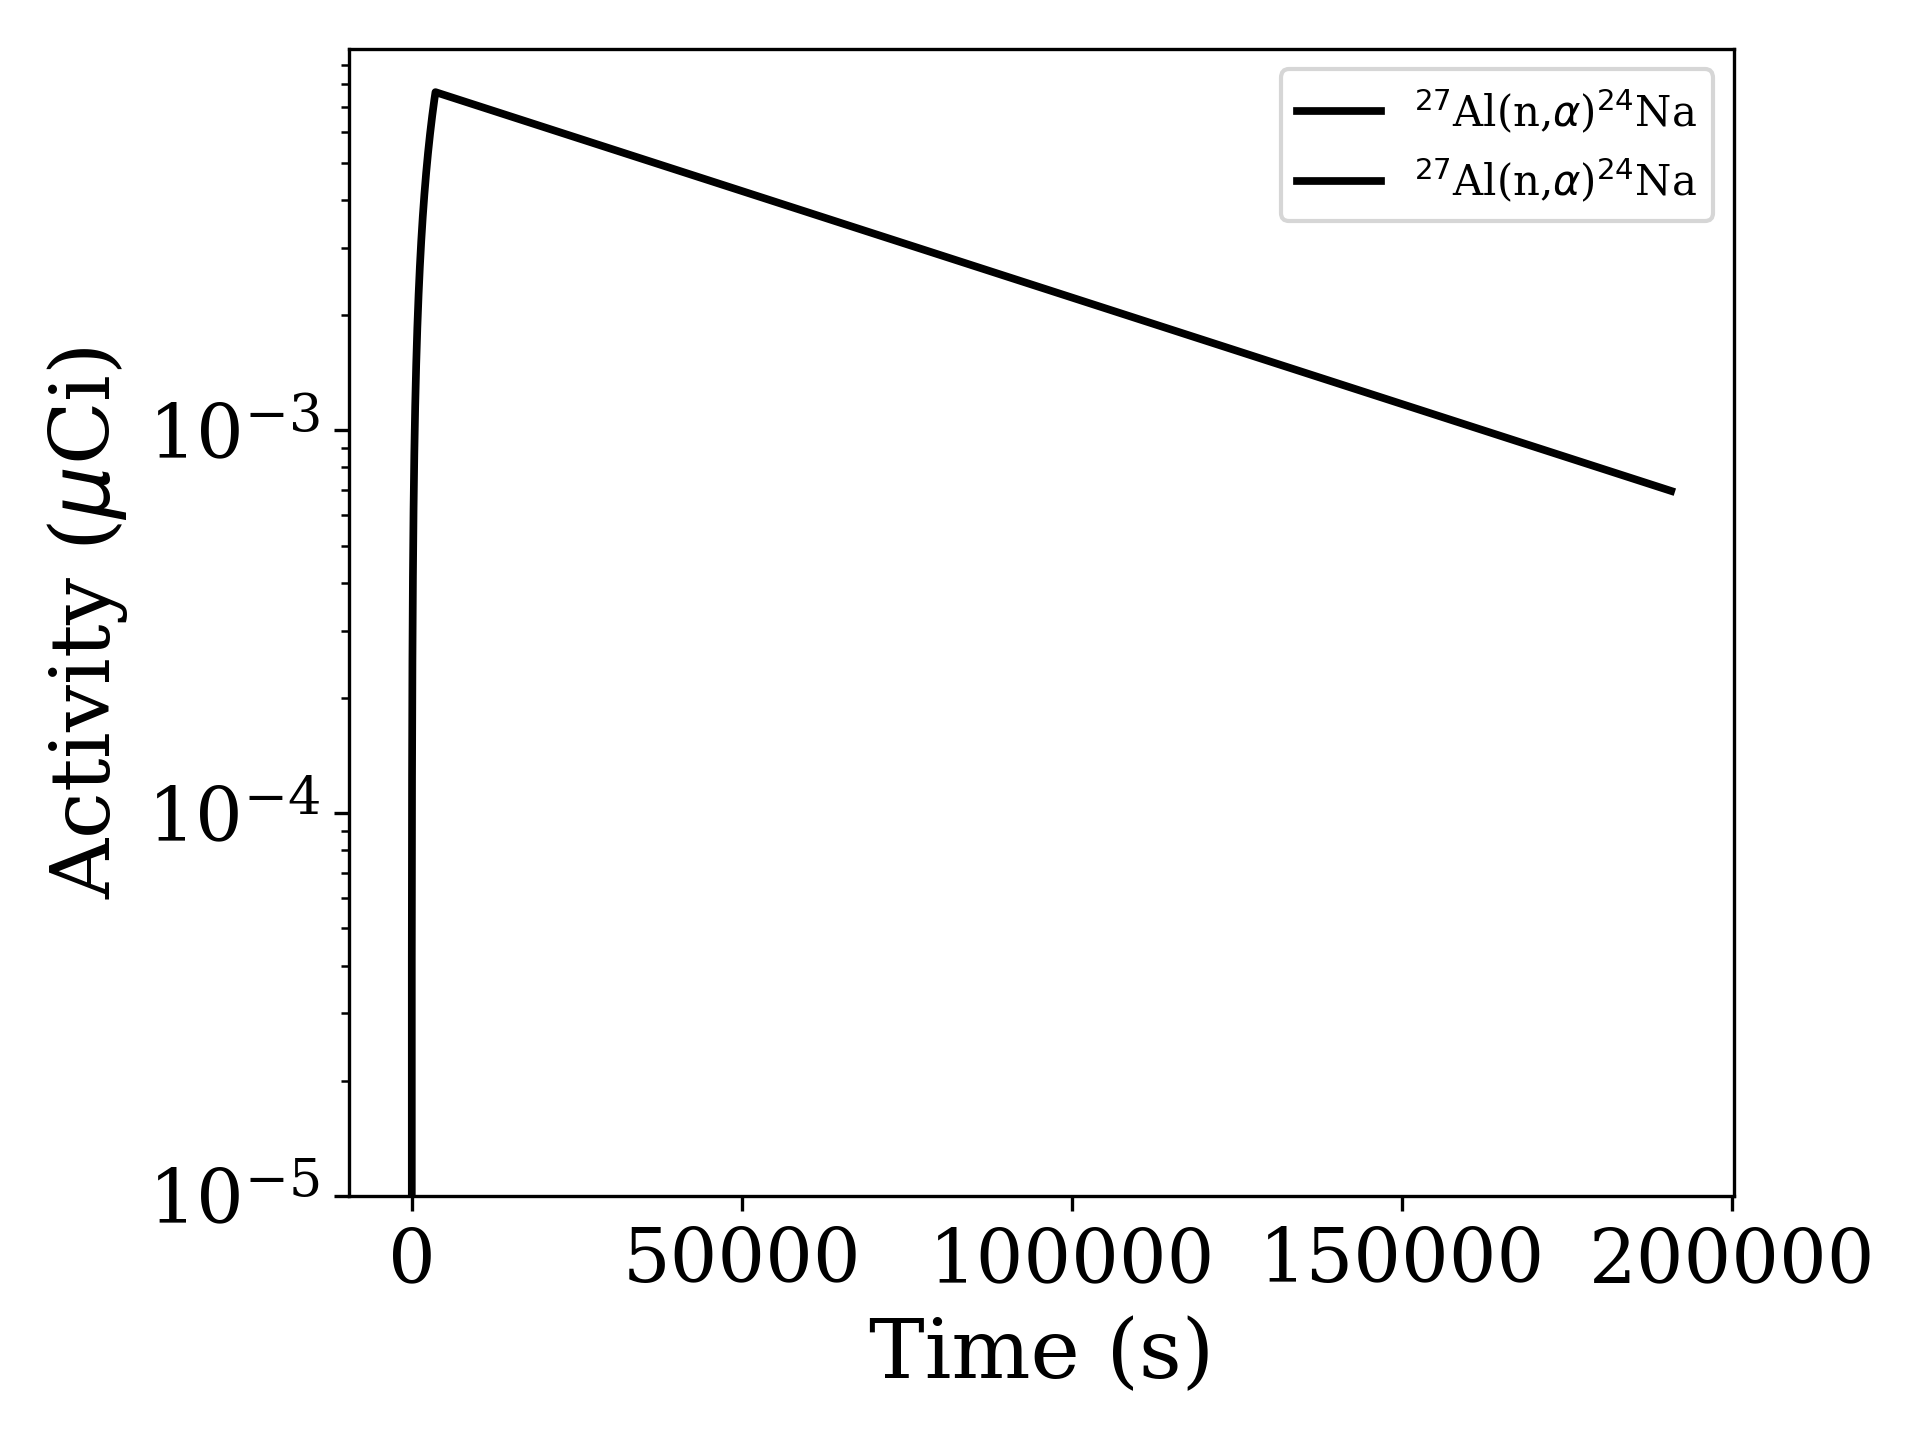
\includegraphics[width=.8\textwidth]{plot/Al-27(n,alpha)Na-24_library1} 

  \caption{A subfigure}
  \label{fig:sub1}
\end{subfigure}%
\begin{subfigure}{.5\textwidth}
  \centering
     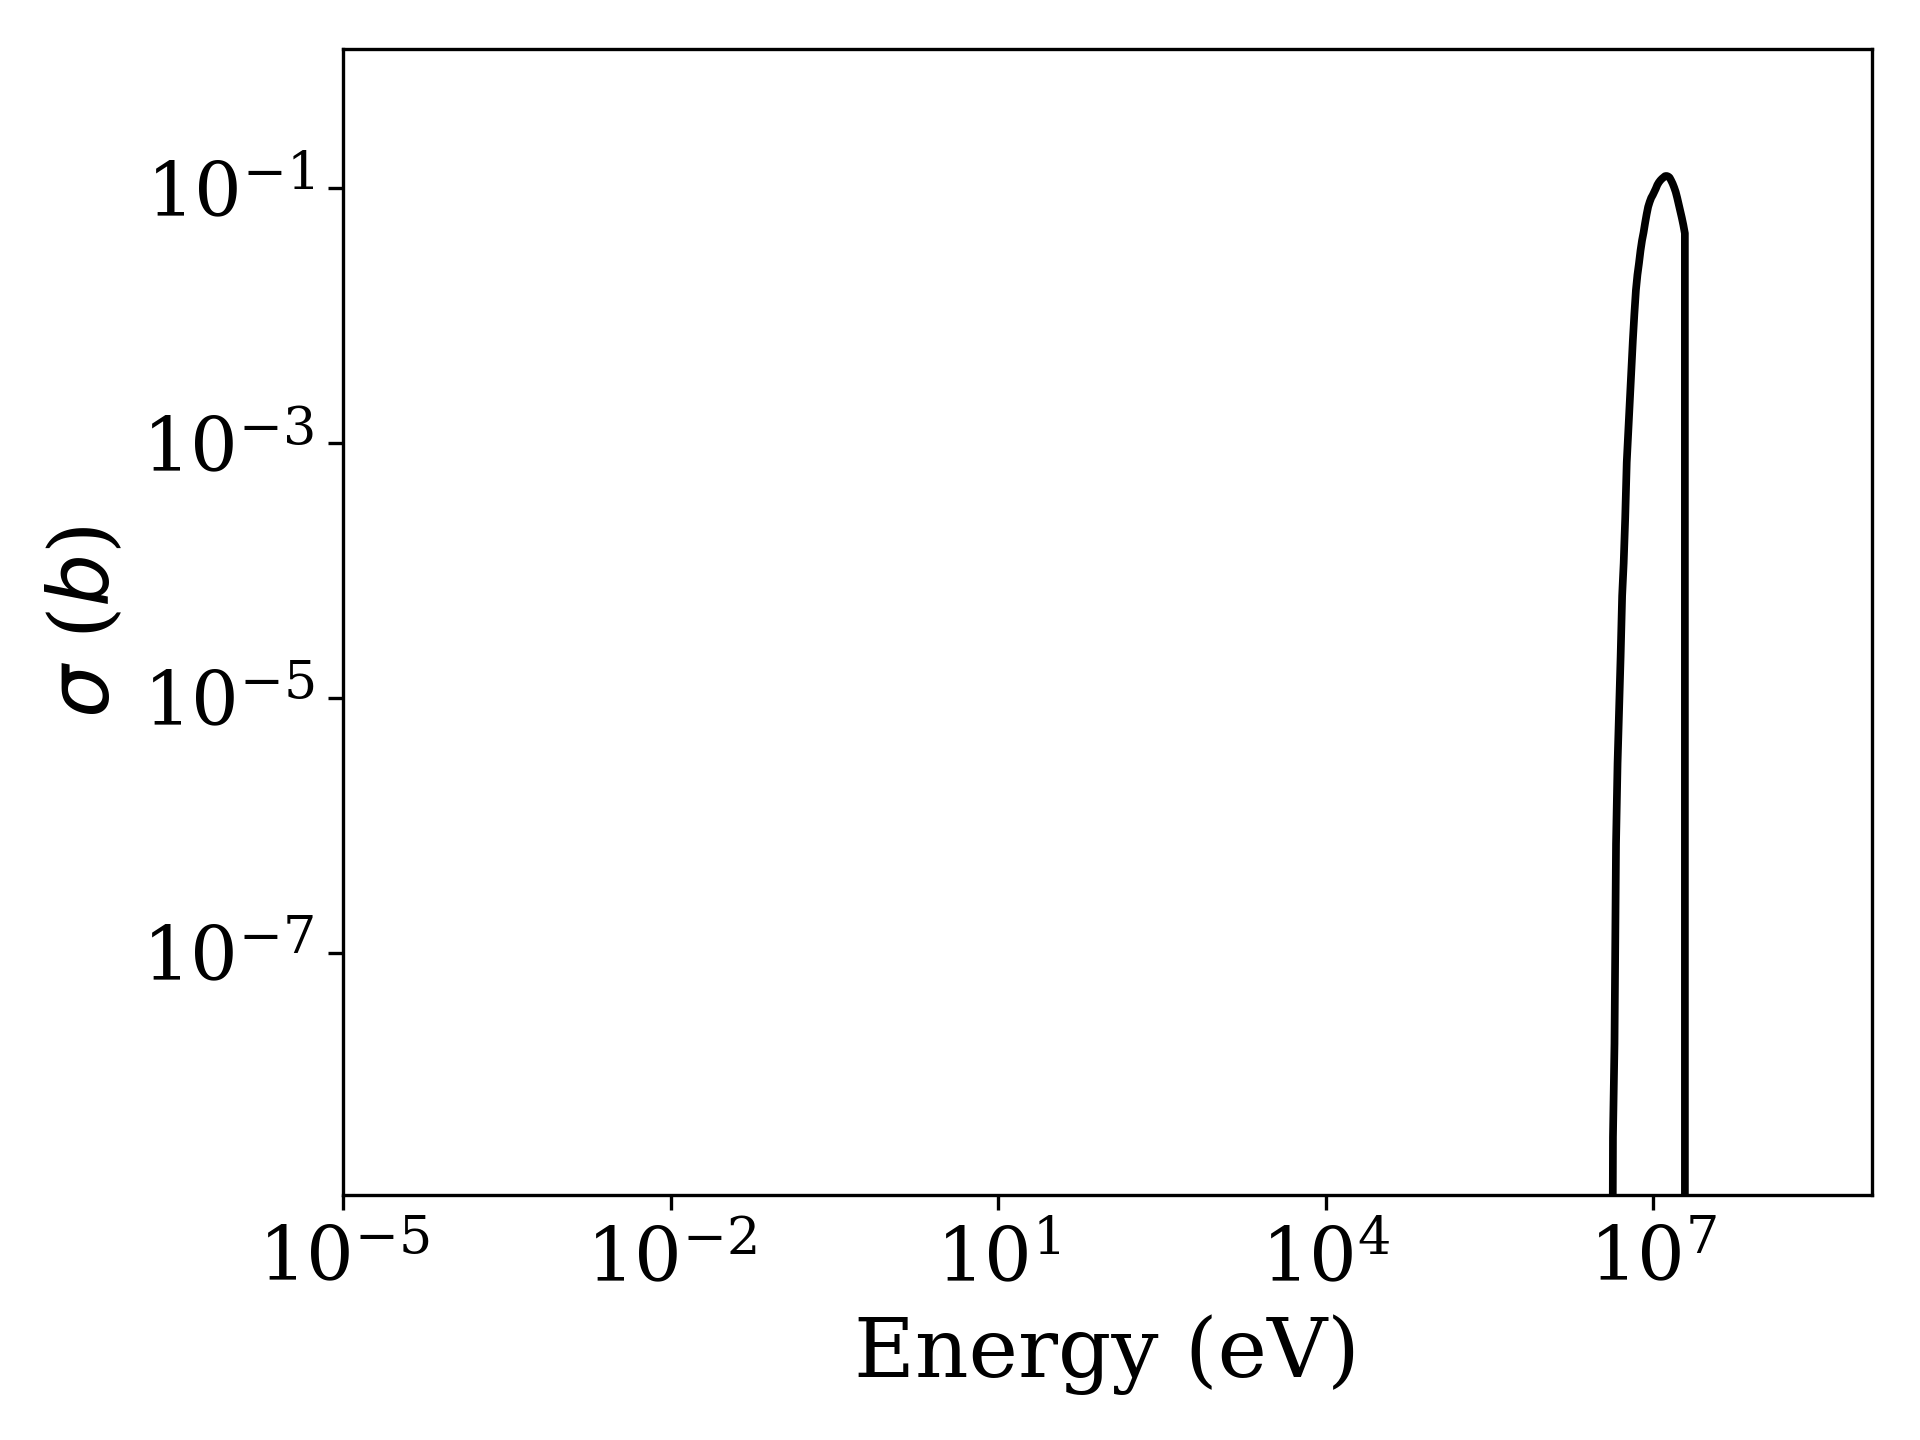
\includegraphics[width=.8\textwidth]{plot/Al-27(n,alpha)Na-24} 

  \caption{A subfigure}
  \label{fig:sub2}
\end{subfigure}
\caption{A figure with two subfigures}
\label{fig:test}
\end{figure}

\begin{table*}[h]
\centering
\begin{tabular}{ |c|c|c|c|c|c|c| }
 \hline
 Reaction & T$_{1/2}$ & ROI (eV) & Important Gammas (keV) \\
 \hline 
 $^{27}$Al(n,$\alpha$)$^{24}$Na & 15.0 h & 6.56e+06, 1.21e+07 & 1368.626(0.999936) \\ 
\hline
\end{tabular}
\end{table*}
